\section{Introduction}

Generative machine learning models have recieved significant attention in recent years due to their capability to synthesize realistic and diverse data samples. Such models learn the probability distributions of real-world datasets and generate new instances. These techniques have numerous applications, including data augmentation, anomaly detection, image restoration, and even medical diagnostics~\cite{yi2019generative}.

In the context of medical imaging, generative approaches have the potential to mitigate common challenges such as limited data availability, imbalanced class distribution, and the high costs associated with obtaining labeled medical data. Specifically, generative models like Generative Adversarial Networks~\cite{goodfellow2014generative} (GANs), Variational Autoencoders~\cite{kingma2013auto} (VAEs), and Diffusion Models~\cite{ho2020denoising} have shown great promise in generating realistic medical images.

In this project, I address the task of synthesizing realistic blood cell images from the BloodMNIST dataset~\cite{medmnistv2}. The BloodMNIST dataset comprises RGB images of peripheral blood smear cells, categorized into eight distinct cell types: neutrophils, eosinophils, basophils, lymphocytes, monocytes, immature granulocytes, erythroblasts, and platelets (Fig.~\ref{fig:bloodmnist_examples}).

\begin{figure}
    \centering
    \begin{minipage}{0.22\textwidth}
        
\includegraphics[width=\linewidth]{images/bloodmnist_classes/neutrophil.png}
        (a) Neutrophil
    \end{minipage}
    \hfill
    \begin{minipage}{0.22\textwidth}
        
\includegraphics[width=\linewidth]{images/bloodmnist_classes/eosinophil.png}
        (b) Eosinophil
    \end{minipage}
    \hfill
    \begin{minipage}{0.22\textwidth}
        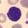
\includegraphics[width=\linewidth]{images/bloodmnist_classes/basophil.png}
        (c) Basophil
    \end{minipage}
    \hfill
    \begin{minipage}{0.22\textwidth}
        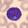
\includegraphics[width=\linewidth]{images/bloodmnist_classes/lymphocyte.png}
        (d) Lymphocyte
    \end{minipage}
    \\[1em]
    \begin{minipage}{0.22\textwidth}
        
\includegraphics[width=\linewidth]{images/bloodmnist_classes/monocyte.png}
        (e) Monocyte
    \end{minipage}
    \hfill
    \begin{minipage}{0.22\textwidth}
        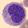
\includegraphics[width=\linewidth]{images/bloodmnist_classes/immature_granulocytes.png}
        (f) I. Granulocyte
    \end{minipage}
    \hfill
    \begin{minipage}{0.22\textwidth}
        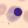
\includegraphics[width=\linewidth]{images/bloodmnist_classes/erythroblast.png}
        (g) Erythroblast
    \end{minipage}
    \hfill
    \begin{minipage}{0.22\textwidth}
        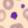
\includegraphics[width=\linewidth]{images/bloodmnist_classes/platelet.png}
        (h) Platelet
    \end{minipage}
    \caption{Examples of each blood cell class from the BloodMNIST dataset.}\label{fig:bloodmnist_examples}
\end{figure}
